% =====================================================================
%  Queyi — NeurIPS 2027 Datasets & Benchmarks submission (anonymous)
%  Migrated from the Chinese working draft (v0.7). All numbers match that draft.
%  Engine: pdflatex/bibtex  (or tectonic).  Style: official neurips_2025.sty
% =====================================================================
\documentclass{article}

\usepackage[dandb]{neurips_2025}   % Datasets & Benchmarks track; anonymous by default
\usepackage[utf8]{inputenc}
\usepackage[T1]{fontenc}
\usepackage{hyperref}
\usepackage{url}
\usepackage{booktabs}
\usepackage{amsfonts}
\usepackage{amsmath}
\usepackage{amssymb}
\usepackage{graphicx}
\usepackage{xcolor}
\usepackage{tikz}
\usepackage{pgfplots}
\pgfplotsset{compat=1.17}
\usetikzlibrary{arrows.meta,positioning,shapes.geometric,fit,backgrounds}

% placeholder for results pending the baseline batch (kept visible on purpose)
\newcommand{\TODO}[1]{\textcolor{red}{\textbf{[TODO: #1]}}}
\newcommand{\cmark}{\textcolor{green!60!black}{\checkmark}}

\title{Queyi: Making Verification Capability\\ Independently Auditable}

\author{%
  Anonymous Author(s) \\
  Affiliation \\
  Address \\
  \texttt{email} \\
}

\begin{document}
\maketitle

\begin{abstract}
LLMs generate technical knowledge (assertions, rules, tutorials) at near-zero cost,
but \emph{verifying} it remains expensive. Two existing routes fail: \textbf{model-judges-model}
puts the verifier and the verified in the same failure domain, and \textbf{AI-text detection}
answers the wrong question---provenance is independent of truth. We present \textbf{Queyi}, a
verification system that binds \emph{conclusion--evidence--recomputation} into a chain that an
external party can interrupt. Its objects are \emph{executable C++ assertions}; its verdict is
\emph{four-state} (\texttt{pass}/\texttt{fail}/\texttt{unknown}/\texttt{contradict}, with
\texttt{unknown} a first-class citizen); and its credibility comes from a forced split of
provenance vs.\ semantic scope, a \emph{kernel-independent} meta-state reconciler, and a
\emph{failure-driven} loop that turns each miss into new verification capability. The current
system has \textbf{67} verdict rules, \textbf{42} real cards, a \textbf{452}-event authority
ledger, and Merkle roots over \textbf{5} controlled directories. \textbf{On the same samples}, blind
holdout recall is \textbf{87.5\% (14/16, 95\% CI [61.7, 98.4])} and corpus measurable recall is
\textbf{43.8\% (14/32, [26.4, 62.3])}, versus a \emph{static caliber arm} at \textbf{6.2\%} and
\textbf{12.5\%} ($\Delta$ \textbf{+81.3pp} / \textbf{+31.3pp}; exact McNemar $p\le0.002$, Cohen's
$h\ge0.72$). \textbf{Limitations:} two headline numbers depend on a
specific WSL sanitizer environment (they fail silently elsewhere); sample sizes are small
($n{=}16/40$); and budget-matched baselines are not yet run---so we claim
\emph{auditability of the mechanism}, \emph{not} superiority over existing methods.
\end{abstract}

% =====================================================================
\section{Introduction}
\label{sec:intro}
% =====================================================================
\paragraph{The problem: generation is easy, verification is not.}
An LLM can emit thousands of C++ technical assertions in minutes. They are \emph{numerous}
(manual review does not scale), \emph{plausible} (syntax, terminology and tone all look right),
and \emph{quietly wrong} (errors surface only under a specific compiler flag, compiler, or
platform). This creates an asymmetry---\textbf{generation cost tends to zero, verification cost
does not}---which is the starting point of this work. Executable evaluation of generated code has
precedent~\cite{chen2021humaneval}; our question differs---not whether code passes tests, but
whether a knowledge claim is true.

\paragraph{Motivation 1: high scores $\neq$ real ability.}
SWE-bench turned ``fix real GitHub issues'' into a standard yardstick~\cite{jimenez2024swebench},
but follow-up work is systematically negative: gains on SWE-bench-Verified are partly
\emph{memory rather than reasoning}---models locate files at up to 76\% within the repo but only
53\% outside it~\cite{liang2025illusion}; models score $3\times$ higher on SWE-bench-Verified
than on two sibling benchmarks~\cite{prathifkumar2025verified}; and SWE-MERA reports 32.67\% of
successful patches involving solution leakage and 31.08\% passing due to insufficient
tests~\cite{adamenko2025swemera}. \emph{Implication:} a verifier tested on its own data will
reproduce this failure, so we choose \textbf{external samples first}, \textbf{irreversible
blinding}, and \textbf{layered reporting}.

\paragraph{Motivation 2: AI-text detection answers the wrong question.}
DetectGPT~\cite{mitchell2023detectgpt} and watermarking~\cite{kirchenbauer2023watermark} answer
``was this text written by an AI?''---a signal that degrades with length/domain and is fragile to
paraphrase~\cite{sadasivan2023canai}. More fundamentally, \textbf{provenance and truth are
independent questions}: human-written C++ can be wrong, and AI-written derivations can be right.
\emph{Implication:} we do not detect provenance; we \textbf{test assertions} (compile, warn,
sanitize, cross-compiler diff, cross-optimization diff).

\paragraph{Motivation 3: provenance moved from good practice to obligation.}
EU Regulation 2024/1689 (AI Act), Article 50 imposes transparency obligations on generative AI
outputs~\cite{eu2024aiact}. This aligns with our design: \textbf{every piece of knowledge must
carry who generated it, who verified it, where the evidence is, and under what conditions it
holds}.

\paragraph{Contributions.}
(1)~\textbf{A verification system} (\S\ref{sec:method}): an
\texttt{artifact}$\to$\texttt{verifier}$\to$\texttt{verdict}$\to$\texttt{ledger} architecture,
four-state verdicts, L0/L1 gate tiers, a forced split of provenance vs.\ semantic scope, a
kernel-independent meta-state reconciler, and the core mechanism---a failure-driven verification
loop.
(2)~\textbf{An evaluation protocol} (\S\ref{sec:protocol}): five dataset layers D0--D4,
three budget-matched baselines, a six-group ablation with pre-registered hypotheses, seven
metrics, and a \emph{frozen} statistical caliber.
(3)~\textbf{An open artifact}: Merkle roots, a transparent log, a 452-event ledger, per-sample
detail artifacts, and single-command recomputation---so that anyone can verify us
\emph{without trusting us}.

\paragraph{What we do \emph{not} claim.}
We do not claim a better C++ textbook, a stronger detector, or a formal proof. We do not claim
``the verifier got stronger'' unless that strengthening is measured on the \emph{same external
samples under the same caliber} (\S\ref{sec:exp}, Fig.~\ref{fig:evolution}).

% =====================================================================
\section{Related Work}
\label{sec:related}
% =====================================================================
We compress prior work into four lines (a seven-direction table is in Appendix~\ref{app:related}).
All comparisons are \emph{positional and qualitative}, not empirical claims about those systems.

\paragraph{(1) Self-evolving / contamination-resistant benchmarks (they evolve the \emph{items}).}
Benchmark Self-Evolving~\cite{wang2024benchmarkevolving}, ArenaBencher~\cite{liu2025arenabencher},
SWE-bench-Live~\cite{zhang2025swebenchlive}, DynaBench~\cite{kiela2021dynabench} and
LiveBench~\cite{white2024livebench} all fight ``the model memorized the items'', but they evolve
the \emph{object under test}; who judges, and whether the judgment is right, remains a fixed
test/oracle.

\paragraph{(2) Mutation-guided LLM test generation (the closest engineering form).}
ACH~\cite{foster2025ach} and MUTGEN~\cite{wang2025mutgen} turn mutation testing from an
\emph{evaluation} device into a \emph{generation} device; Cleverest~\cite{liu2025cleverest} does
just-in-time regression test generation. We \emph{reuse} the mutation-feedback idea as an internal
self-justification layer, but we \emph{refuse} to treat mutation score as a defect-detection rate.

\paragraph{(3) Self-verification / LLM-as-a-judge / formal verification (partly adopted, partly rejected).}
LLM-as-a-judge~\cite{zheng2023judging} is practical and scalable, but we use LLMs only to
\emph{propose candidates} and keep the \emph{judgment} fully programmatic. seL4~\cite{klein2009sel4}
and CompCert~\cite{leroy2009compcert} show that proof power can be extreme, at high human cost and
narrow coverage; we do not pursue formal proofs, only \emph{evidence that a third party can
recompute line by line}. The mutation-testing survey~\cite{jia2011mutation} informs our framework,
but only for the self-justification layer.

\paragraph{(4) Measurement governance, reproducibility, provenance (our methodological sources).}
Goodhart/Strathern~\cite{goodhart1975problems,strathern1997improving}, reward
hacking~\cite{skalse2022rewardhacking}, reward over-optimization~\cite{gao2023scaling};
Datasheets~\cite{gebru2021datasheets} and Model Cards~\cite{mitchell2019modelcards};
reproducibility reporting~\cite{pineau2021improving}; statistical methods~\cite{clopper1934use,
fisher1935design,mcnemar1947note,benjamini1995controlling,holm1979simple,cohen1960coefficient};
Merkle trees~\cite{merkle1988digital} and provenance auditing~\cite{kao2025constantsize,wang2026whoaudits}.

\begin{table}[t]
\caption{Positioning. Benchmark evolution evolves \emph{items}; mutation-guided testing evolves
\emph{tests}; formal verification provides \emph{proofs}; Queyi evolves the \emph{measuring stick}
(verdict and evidence-acquisition capability) while requiring that this change be externally
measurable.}
\label{tab:positioning}
\centering
\small
\begin{tabular}{@{}p{2.4cm}p{2.6cm}p{2.6cm}p{2.6cm}p{3.4cm}@{}}
\toprule
 & Benchmark evol. & Mutation-guided & Formal verification & \textbf{Queyi (ours)} \\
\midrule
Object evolved & items / samples & tests \& mutants & proofs (static) & \textbf{verdict + evidence capability} \\
Who judges & fixed test/judge & fixed oracle & proof checker & \textbf{programmatic rules + 4-state + reconciler} \\
Can say ``unknown'' & usually no & usually no & n/a & \textbf{yes (\texttt{unknown} first-class)} \\
Meaning of a gain & model stronger & suite stronger & no score & \textbf{verification capability} \\
Anti-gaming & new items & new mutants & n/a & \textbf{failure-driven + blind + budget-matched} \\
\bottomrule
\end{tabular}
\end{table}

\paragraph{What we are not.} Not benchmark evolution (we evolve the stick, not the items); not
mutation testing (mutation is only an internal self-justification component); not
self-verification (judgment is fully programmatic; meta-state is checked by an independent
reconciler); not RAG/text-similarity (we verify \emph{executable assertions}, not textual
resemblance).

% =====================================================================
\section{Problem Definition and Threat Model}
\label{sec:threat}
% =====================================================================
\paragraph{Formalization.}
A \emph{knowledge assertion} $a$ is a decidable statement plus a \emph{boundary triple}
$\langle D, P, F\rangle$ (input domain, preconditions, failure conditions). \emph{Evidence} $e$ is
a replayable observation (compiler version $+$ command $+$ optimization level $+$ output $+$
content-addressed hash). A \emph{verdict} is $v\in\{\texttt{pass},\texttt{fail},\texttt{unknown},
\texttt{contradict}\}$; \emph{verification capability} $\mathcal{C}$ is the set of available
evidence-acquisition means. Our goal is \textbf{not} to maximize $\Pr[v{=}\texttt{pass}]$ but to
maximize agreement with ground truth \emph{without ever disguising \texttt{unknown} as \texttt{pass}}.

\paragraph{Why four states.} ``Detector unavailable'' and ``detector says fine'' are different
knowledge states. Recording \texttt{unknown} as \texttt{miss} understates capability and pollutes
the denominator; as \texttt{pass} it creates a \emph{false pass} (the most dangerous); recording
\texttt{miss} as \texttt{unknown} hides a capability gap. Hence the \textbf{denominator is
$\text{catch}+\text{miss}$ (measurable samples)}; \texttt{unknown} is reported separately and
excluded; \texttt{not\_error} is a separate class. The caliber is stored in the artifact, not in
prose.

\paragraph{Twelve threats (T1--T12).}
Table~\ref{tab:threats} lists them; \S\ref{sec:validity} quantifies them under the standard
validity layers~\cite{shadish2002experimental}.

\begin{table}[t]
\caption{Threats, mitigations and residual risks.}
\label{tab:threats}
\centering
\small
\begin{tabular}{@{}p{0.5cm}p{4.6cm}p{4.2cm}p{4.6cm}@{}}
\toprule
\# & Threat & Mitigation & Residual \\
\midrule
T1 & Self-justification (toolchain proves itself) & kernel-independent reconciler (\S\ref{sec:reconciler}) & reconciler still needs human review; \texttt{--check} $\neq$ independent implementation \\
T2 & Self-made distribution bias & blind holdout + external corpus (D2/D3) & small external sample \\
T3 & holdout leakage & irreversible reveal; holdout dir not scanned & 10 appended samples have no blinding \\
T4 & developer-knowledge bias & independent generation (A/B/C) & same-process context; not truly independent \\
T5 & caliber drift & meta-state reconciliation & covers registered fields only \\
T6 & semantic-scope misuse & forced provenance/scope split (\S\ref{sec:prov}) & scope completeness 0/26 \\
T7 & metric confusion (mutation $\to$ detection) & metric layering; mutation is self-justification only & external readers may still misread \\
T8 & selection bias (budget) & budget-matched random baseline (\S\ref{sec:baseline}) & not yet run \\
T9 & overfitting historical defects & blind D2 + external D3 & appended samples unblinded \\
T10 & reproducibility crisis & Merkle roots + version capture + time anchor & OTS is a placeholder; WSL dependency undeclared \\
T11 & authority manipulation & 452-event ledger, zero-change red line & discipline, not cryptographic enforcement \\
T12 & unclear AI authorship & AI-use registry & contribution split remains a convention \\
\bottomrule
\end{tabular}
\end{table}

\paragraph{Three focus threats.}
\textbf{(a) Construct: ``execution passed'' $\neq$ ``knowledge is correct.''} A \texttt{catch}
means only that a specific signal appeared under a specific fixture, flag and compiler---not that
the assertion is true or false. Empirically, the same ASan samples are optimized away under
\texttt{-O1} (no observable side effect) and reported immediately under \texttt{-O0}; switching the
pipeline from single- to dual-flag (\texttt{-O0}+\texttt{-O2}) moved recall \textbf{66.7\% $\to$
87.5\% with the detector unchanged}---\emph{the caliber changed, not the capability}.
\textbf{(b) Meta-Goodhart: the verifier optimizes its own metric.} When the \emph{measure of
verification capability} is produced by the verification system, the system can raise its score by
changing the caliber, changing the denominator, or turning red lights green, with no external
reference. A real incident: a batch changed the detector flag but \emph{did not rerun the
generator}; the artifact stayed on the old caliber while the paper reported \textbf{81.2\%
(13/16)}---a number that \emph{never appeared in any artifact}---and the then-\texttt{--check} did
not compare those fields, so it stayed green. \textbf{(c) Evaluation contamination.} Three forms:
sample leakage (T3); \emph{shared-criterion} labeling, where ground-truth labels and the criterion
are generated by the same rule, making the score an \emph{upper bound} (our counterfactual
operator's $F_1{=}1.0$); and unblinded expansion.

% =====================================================================
\section{Method}
\label{sec:method}
% =====================================================================
\begin{figure}[t]
\centering
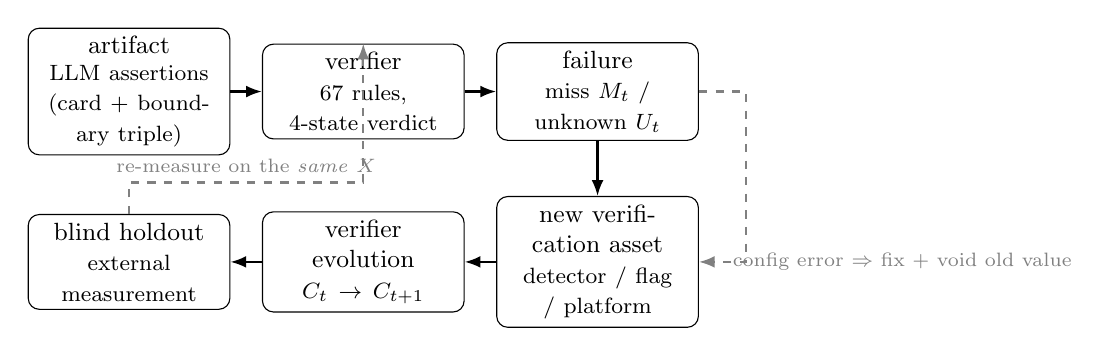
\begin{tikzpicture}[
  font=\small,
  box/.style={draw, rounded corners, align=center, inner sep=3pt, minimum height=9mm, text width=2.35cm},
  arr/.style={-{Latex[length=2mm]}, thick},
  fb/.style={-{Latex[length=2mm]}, dashed, thick, gray}
]
\node[box] (a) {artifact\\\footnotesize LLM assertions\\\footnotesize (card + boundary triple)};
\node[box, right=4mm of a] (b) {verifier\\\footnotesize 67 rules, 4-state verdict};
\node[box, right=4mm of b] (c) {failure\\\footnotesize miss $M_t$ / unknown $U_t$};
\node[box, below=7mm of c] (d) {new verification asset\\\footnotesize detector / flag / platform};
\node[box, left=4mm of d] (e) {verifier evolution\\\footnotesize $C_t \to C_{t+1}$};
\node[box, left=4mm of e] (f) {blind holdout\\\footnotesize external measurement};
\draw[arr] (a)--(b);
\draw[arr] (b)--(c);
\draw[arr] (c)--(d);
\draw[arr] (d)--(e);
\draw[arr] (e)--(f);
\draw[fb] (f.north) -- ++(0,4mm) -| node[pos=0.25, above, font=\scriptsize]{re-measure on the \emph{same} $X$} (b.north);
\draw[fb] (c.east) -- ++(6mm,0) |- node[pos=0.75, right, font=\scriptsize, align=left]{config error $\Rightarrow$ fix + void old value} (d.east);
\end{tikzpicture}
\caption{The failure-driven verification loop. Solid arrows form the main cycle; dashed arrows
are re-measurement and caliber correction. Tools: the rule engine (67 rules, four states), the
kernel-independent meta-state reconciler, and the counterfactual operator.}
\label{fig:loop}
\end{figure}

\paragraph{Architecture.}
\texttt{artifact}$\to$\texttt{verifier}$\to$\texttt{verdict}$\to$\texttt{ledger} (Fig.~\ref{fig:loop}).
\emph{Artifact}: knowledge cards, each with a boundary triple; a card lacking the triple may not
be pre-assigned a verdict (it should be \texttt{unknown}---a \emph{correct} output).
\emph{Verifier}: \textbf{67} rules produce four-state verdicts (two sources agree: engine rules
$=$ rule manifest). \emph{Evidence}: each compile/run stores content-addressed evidence (version
$+$ command $+$ flag $+$ output $+$ sha256); currently \textbf{28} cards have L1 evidence,
\textbf{28} are double-compiler confirmed, over \textbf{147} real compilations. \emph{Ledger}: a
\textbf{452}-event append-only authority ledger under a zero-change red line.

\paragraph{Four-state verdict.}
\begin{table}[t]
\caption{Four-state verdict.}
\label{tab:verdict}
\centering
\small
\begin{tabular}{@{}lll@{}}
\toprule
State & Meaning & Action \\
\midrule
\texttt{pass} & evidence supports the assertion; boundary triple complete & may enter the teaching ledger \\
\texttt{fail} & evidence contradicts the assertion & counterexample to the teaching set \\
\texttt{unknown} & insufficient evidence or detector unavailable & never recorded as pass/miss; reported separately \\
\texttt{contradict} & two pieces of evidence conflict (e.g.\ cross-compiler) & escalated to human review; no machine pick \\
\bottomrule
\end{tabular}
\end{table}
The point of \texttt{contradict} is that \emph{the machine never picks a side when evidence
conflicts}---the conflict itself is information. Machine cards are always
\texttt{needs\_review}$=$true and never counted as ``verified''; \texttt{verified} is
human-signed only.

\paragraph{Gate tiers L0/L1.} \textbf{L0 (blocking)}: meta-state reconciliation, gate-tier
legality, real-defect detection, blind-holdout state, unit tests---\textbf{7} L0 gates; the
orchestrator's 5 stages all PASS stage-by-stage in the audit. \textbf{L1 (advisory)}: mutation
score, boundary provenance report, supply-chain integrity---\textbf{10} L1 gates; red is not
blocking but must be registered. Tiering separates ``must hold'' from ``up for discussion'';
putting everything at L0 invites relaxing assertions to go green.

\paragraph{Provenance vs.\ semantic scope (forced split).}
\label{sec:prov}
\emph{Provenance} answers \emph{where an assertion comes from / who generated it} (generator
version, mutation-set hash, evidence sha256, compiler version). \emph{Semantic scope} answers
\emph{where it holds} (standard clause / compiler / platform / optimization level). They must be
split because a provenance-complete assertion can still be misused outside its scope (T6); writing
them together invites ``clear origin $\Rightarrow$ holds everywhere''. Current state (audit):
\textbf{26} boundary cards, provenance complete \textbf{26/26}, \textbf{semantic scope complete
0/26}---the mechanism is in place but scope backfill is essentially empty, which directly limits
external validity.

\paragraph{Meta-state reconciler (anti-self-justification).}
\label{sec:reconciler}
The reconciler is \emph{kernel-independent}: it rescans the ground-truth sources (card fields,
directories, the rule engine) and compares them with the baseline, emitting
\texttt{META-STATE-CONFLICT} and exiting 1 on mismatch. Its own discipline: assertions may
hard-code a \emph{caliber}, never a \emph{measurement}---via (i) ground-truth alignment
(recompute), (ii) additivity/partition (\texttt{block}$+$\texttt{warn}$+$\texttt{advice}$=$total),
or (iii) structural invariants. Residual: ``kernel-independent'' means it does not import the
kernel, \emph{not} that it is a third-party implementation.

\paragraph{Failure-driven loop.} For every \texttt{miss}$\cup$\texttt{unknown}, attribute the
cause: a \emph{measurement-configuration error} (fix the config and \emph{void the old value}---not
a capability gain) or a \emph{capability gap} (add an evidence-acquisition means $\Rightarrow
C_{t+1}$); then \textbf{re-measure on the same $X$} and quantify $\Delta$ with a CI; if $\Delta$ is
not significant, the capability addition does \emph{not} enter the claim table. Re-measuring on the
same $X$ is essential---otherwise ``capability gain'' is indistinguishable from ``an easier sample
set''. A budget-matched random control is essential because failure-driven gains may simply reflect
\emph{more budget}.

% =====================================================================
\section{Evaluation Protocol}
\label{sec:protocol}
% =====================================================================
The protocol is \emph{frozen before seeing results}; later changes must be logged with their effect
on existing numbers. Statistical details are in Appendix~\ref{app:stats}.

\begin{figure}[t]
\centering
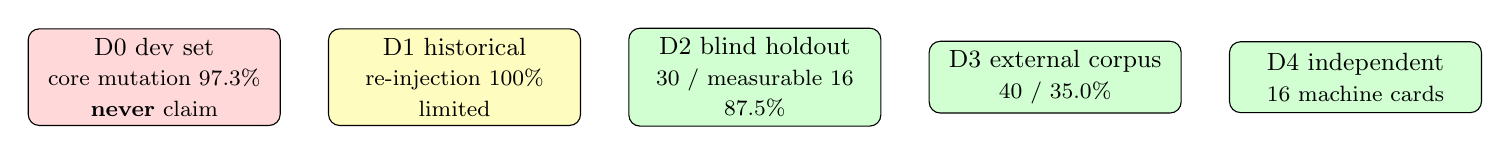
\begin{tikzpicture}[font=\small]
\node[draw, rounded corners, fill=red!15, align=center, minimum width=3.2cm, minimum height=9mm] (d0) {D0 dev set\\\footnotesize core mutation 97.3\%\\\footnotesize \textbf{never} claim};
\node[draw, rounded corners, fill=yellow!25, align=center, minimum width=3.2cm, minimum height=9mm, right=6mm of d0] (d1) {D1 historical\\\footnotesize re-injection 100\%\\\footnotesize limited};
\node[draw, rounded corners, fill=green!18, align=center, minimum width=3.2cm, minimum height=9mm, right=6mm of d1] (d2) {D2 blind holdout\\\footnotesize 30 / measurable 16\\\footnotesize 87.5\%};
\node[draw, rounded corners, fill=green!18, align=center, minimum width=3.2cm, minimum height=9mm, right=6mm of d2] (d3) {D3 external corpus\\\footnotesize 40 / 35.0\%};
\node[draw, rounded corners, fill=green!18, align=center, minimum width=3.2cm, minimum height=9mm, right=6mm of d3] (d4) {D4 independent\\\footnotesize 16 machine cards};
\end{tikzpicture}
\caption{Dataset layers D0--D4. Colour encodes whether external validity may be claimed
(red: never; yellow: limited; green: yes). D0 is self-justification only; D2 contains 10 unblinded
samples (denominator only); D3 is further split into layers A/B/C which must \emph{not} be merged.}
\label{fig:data}
\end{figure}

\paragraph{Dataset layers (D0--D4).}
\begin{table}[t]
\caption{Five dataset layers.}
\label{tab:data}
\centering
\small
\begin{tabular}{@{}lp{3.4cm}p{3.2cm}p{2.4cm}p{3.4cm}@{}}
\toprule
Layer & Content & Use & External valid.? & Current \\
\midrule
D0 dev & internal mutants & tuning / self-justification & \textbf{never} & core mutation 97.3\% \\
D1 historical & known fixed defects (re-injected) & real-defect recall & limited (seen) & re-injection 1/1; coverage 12/15 \\
D2 blind holdout & planted defects, invisible pre-reveal & \textbf{blind recall (main)} & yes & 30 samples; 16 measurable; \textbf{87.5\%} \\
D3 external corpus & real statements from outside the repo & \textbf{external recall (main)} & yes & 40 items; \textbf{35.0\%} \\
D4 independent & assertions from an independent pipeline & independent-generation recall & yes & 16 machine cards (unsigned) \\
\bottomrule
\end{tabular}
\end{table}

\paragraph{Baselines (three, all budget-matched).}
\label{sec:baseline}
\begin{table}[t]
\caption{Baselines and their alignment conditions.}
\label{tab:baseline}
\centering
\small
\begin{tabular}{@{}lp{5.2cm}p{6.4cm}@{}}
\toprule
Baseline & Definition & Alignment \\
\midrule
B1 static gate & static rules only (no runtime evidence) & same corpus, same verdict granularity \\
B2 static $+$ mutation & static rules $+$ mutation testing & same as above $+$ same mutation budget \\
\textbf{B3 budget-matched random} & random evidence acquisition under \emph{equal budget} & same budget (time/calls), same corpus, same flags \\
\bottomrule
\end{tabular}
\end{table}
B3 is the key control: it separates ``failure-driven'' from ``it just spends more''.
\textbf{Current status: 0 baselines run}---the largest experimental gap.

\paragraph{Ablation (A--F, pre-registered hypotheses).}
\begin{table}[t]
\caption{Ablation groups.}
\label{tab:ablation}
\centering
\small
\begin{tabular}{@{}clp{5.6cm}p{3.4cm}@{}}
\toprule
Group & Remove/change & Pre-registered hypothesis & Primary metric \\
\midrule
A & Full & baseline & blind + external recall \\
B & $-$mutation & external recall \emph{unchanged} & external-recall difference $+$ CI \\
C & $-$Merkle & recomputability drops; recall unchanged & number of repro failures \\
D & $-$evidence layer & \texttt{unknown} rate \emph{rises} & \texttt{unknown} rate \\
E & $-$boundary enforcement & \emph{false-pass} rate rises & false-pass rate \\
F & random-budget control & if gains come from ``more attempts'', random catches up & same-budget recall \\
\bottomrule
\end{tabular}
\end{table}
Each group writes its hypothesis before results; a result contradicting the hypothesis is reported
as-is. \textbf{Current status: 0 groups run.}

\paragraph{Metrics (seven).} Real-defect recall; blind-holdout recall; external recall; FPR;
mutation score (\emph{self-justification only}); regression-retention rate; cost. \textbf{Every
rate must carry a \texttt{denominator}}.

% =====================================================================
\section{Experiments}
\label{sec:exp}
% =====================================================================
All numbers are \emph{recomputed from artifacts}; intervals are \textbf{Clopper--Pearson 95\%},
Wilson shown as sensitivity. Baseline arms are recomputed by a single script (see Appendix~\ref{app:repro}).

\begin{figure}[t]
\centering
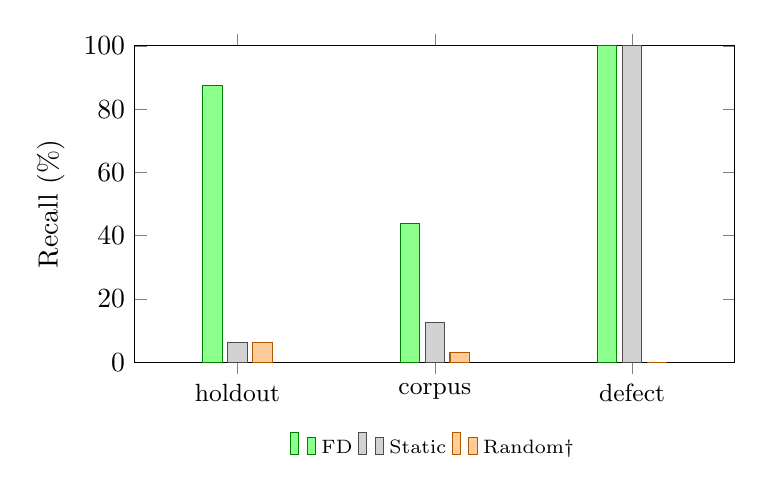
\begin{tikzpicture}
\begin{axis}[
  width=9.2cm, height=5.6cm,
  ybar, bar width=7pt,
  ymin=0, ymax=100,
  ylabel={Recall (\%)},
  symbolic x coords={holdout, corpus, defect},
  xtick=data,
  x tick label style={font=\small},
  legend style={font=\scriptsize, at={(0.5,-0.20)}, anchor=north, legend columns=3, draw=none},
  enlarge x limits=0.26,
  title style={font=\small},
]
\addplot[fill=green!45, draw=green!50!black] coordinates {(holdout,87.5) (corpus,43.8) (defect,100)};
\addplot[fill=gray!35, draw=gray!60!black] coordinates {(holdout,6.2) (corpus,12.5) (defect,100)};
\addplot[fill=orange!40, draw=orange!70!black] coordinates {(holdout,6.2) (corpus,3.1) (defect,0)};
\legend{FD, Static, Random$\dagger$}
\end{axis}
\end{tikzpicture}
\caption{Core recall across three arms. \textbf{FD} (failure-driven) holdout
87.5\% [61.7, 98.4] and corpus 43.8\% [26.4, 62.3]; \textbf{Static} (rule-only, a
\emph{caliber re-binning}, not a re-run) 6.2\% [0.2, 30.2] / 12.5\% [3.5, 29.0];
\textbf{Random$\dagger$} (an instrument-level \emph{proxy}, not the paper's B3) 6.2\% / 3.1\%.
Bars show point estimates; Clopper--Pearson 95\% CIs are in Table~\ref{tab:e1}. $n=16/32$ is
small, so read \emph{direction}, not magnitude.}
\label{fig:core}
\end{figure}

\paragraph{E1 --- Main experiment: static vs.\ random vs.\ failure-driven.}
\begin{table}[t]
\caption{E1. Three arms on the same samples. Static is a caliber re-binning; Random$\dagger$ is a
proxy (the real B3 needs the split-repo \texttt{select\_assets}).}
\label{tab:e1}
\centering
\small
\begin{tabular}{@{}lp{2.7cm}p{2.4cm}p{1.7cm}p{1.5cm}@{}}
\toprule
System & Blind holdout (CP 95\%) & Corpus meas.\ (CP 95\%) & Defect & Control FPR \\
\midrule
Static (caliber re-bin) & 6.2\% (1/16) [0.2, 30.2] & 12.5\% (4/32) [3.5, 29.0] & 100\% (6/6) & --- \\
Random$\dagger$ (proxy) & 6.2\% (1/16) [0.2, 30.2] & 3.1\% (1/32) [0.1, 16.2] & N/A & --- \\
\textbf{FD (failure-driven)} & \textbf{87.5\% (14/16) [61.7, 98.4]} & \textbf{43.8\% (14/32) [26.4, 62.3]} & 100\% (6/6) & 11.1\% (1/9) \\
$\Delta$(static$\to$FD) & \textbf{+81.3pp} & \textbf{+31.3pp} & 0 & --- \\
$\Delta$(random$\dagger\to$FD) & \textbf{+81.3pp} & \textbf{+40.7pp} & N/A & --- \\
\bottomrule
\end{tabular}
\end{table}
\textbf{Pre-registered rule:} if the difference CI crosses 0 for Full$-$B1 or Full$-$F, the
``failure-driven'' mechanism does \emph{not} hold and must be reported as-is.

\paragraph{E2 --- Caliber ablation.} Three arms share the \emph{same raw counts} (catch $=14$) and
differ only in the denominator:
\begin{table}[t]
\caption{E2. Caliber ablation (same raw counts, different denominator).}
\label{tab:e2}
\centering
\small
\begin{tabular}{@{}lp{3.6cm}p{3.6cm}p{3.6cm}@{}}
\toprule
Arm & Caliber & holdout (CP 95\%) & external (CP 95\%) \\
\midrule
\textbf{A (main; drop unknown)} & denominator $=$ catch$+$miss & \textbf{87.5\% (14/16) [61.7, 98.4]} & \textbf{43.8\% (14/32) [26.4, 62.3]} \\
B (unknown $\to$ miss) & denominator incl.\ detector-unknown & 82.4\% (14/17) [56.6, 96.2] & 37.8\% (14/37) [22.5, 55.2] \\
C (unknown $+$ not\_error) & denominator $=$ all samples & 82.4\% (14/17) & 35.0\% (14/40) [20.6, 51.7] \\
\midrule
$\Delta$(A$-$C) & & $+5.1$pp & $\mathbf{+8.8}$pp \\
\bottomrule
\end{tabular}
\end{table}
The caliber effect on the external corpus (up to \textbf{8.8}pp) exceeds some inter-layer
differences, so reporting a rate without its caliber lets readers pick anywhere in 35.0--43.8\%.

\begin{figure}[t]
\centering
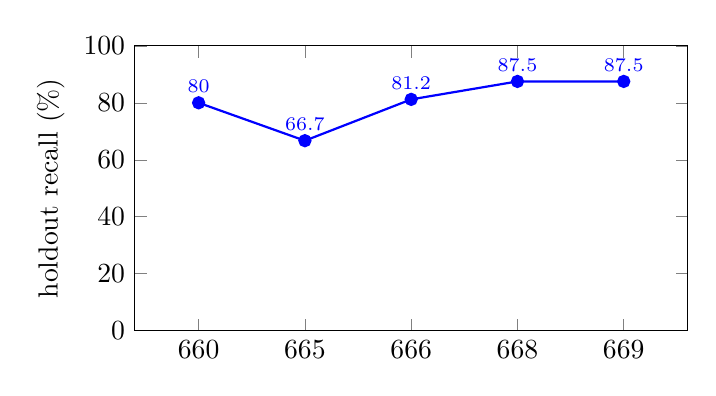
\begin{tikzpicture}
\begin{axis}[
  width=8.6cm, height=5.2cm,
  ymin=0, ymax=100, ylabel={holdout recall (\%)},
  symbolic x coords={660,665,666,668,669}, xtick=data,
  nodes near coords, nodes near coords style={font=\scriptsize},
  enlarge x limits=0.15,
]
\addplot[mark=*, thick, blue] coordinates {(660,80.0) (665,66.7) (666,81.2) (668,87.5) (669,87.5)};
\end{axis}
\end{tikzpicture}
\caption{Evolution curve. \textbf{80.0\% $\to$ 66.7\% $\to$ 87.5\% is not a capability gain}:
660 is a small denominator (20 samples / 7 true errors), 665 is single-flag (30 samples / 17 true
errors), 668 is dual-flag---with the detector unchanged. The 666 value (81.2\%) never landed in
any artifact and is marked hollow. 656/662 report only mutation metrics (core 62.5\% $\to$ 97.3\%).}
\label{fig:evolution}
\end{figure}

\paragraph{E3 --- Evolution curve.}
\begin{table}[t]
\caption{E3. Cross-batch key metrics.}
\label{tab:e3}
\centering
\small
\begin{tabular}{@{}llp{3.0cm}lp{3.0cm}@{}}
\toprule
Batch & New capability & holdout (true/caliber) & mutation core & Nature \\
\midrule
656 & core PBT/mutation & --- & \textbf{62.5\%} (30/48) & mutants out of range \\
660 & trace layer & true 7, \textbf{80.0\%} (small den.) & --- & label over-claim \\
665 & expand 20$\to$30 & true 17, \textbf{66.7\%} (single flag) & --- & denominator changed \\
666 & claimed dual & \textit{81.2\% never landed} & --- & code changed, no rerun \\
668 & dual-flag rerun & \textbf{87.5\%} (14/16) & --- & \textbf{caliber change} \\
669 & caliber ablation $+$ CI & 87.5\% [61.7, 98.4] & \textbf{97.3\%} (110/113) & mutation still internal \\
\bottomrule
\end{tabular}
\end{table}
The holdout column is \emph{not the same $X$}, so it must not be read as evolution. The only
same-sample re-measurement is 668 vs.\ 665, and it changed the \emph{flag}, not the capability.

\paragraph{E4 --- Ablation framework (A0--A5; design frozen, experiments \emph{not} run).}
We re-express the pre-registered ablations as six \emph{same-batch-executable} groups A0--A5, each
with a written hypothesis (H) and a decision rule. Results are \emph{registered} as
\texttt{\{\{TODO\_ablation\_A0\}\}} \dots{} \texttt{\{\{TODO\_ablation\_A5\}\}}: this batch froze the
design and the scripts, it did \textbf{not} run the groups.
\begin{table}[t]
\caption{E4. Ablation groups A0--A5. Each row writes its hypothesis \emph{before} results.}
\label{tab:e4}
\centering
\small
\begin{tabular}{@{}clp{3.3cm}p{3.6cm}l@{}}
\toprule
ID & Remove/change & Hypothesis & Primary metric & Result \\
\midrule
A0 & Full system (baseline) & --- & detection rate & \texttt{\{\{TODO\_ablation\_A0\}\}} \\
A1 & $-$failure-derived rules & H: detection drops & $\Delta$ detection vs.\ A0 & \texttt{\{\{TODO\_ablation\_A1\}\}} \\
A2 & new blind split & H: recall stable & $\Delta$ recall vs.\ A0 & \texttt{\{\{TODO\_ablation\_A2\}\}} \\
A3 & $-$evidence layer & H: \texttt{unknown} rises & \texttt{unknown} rate & \texttt{\{\{TODO\_ablation\_A3\}\}} \\
A4 & $-$boundary enforcement & H: false-pass rises & false-pass rate & \texttt{\{\{TODO\_ablation\_A4\}\}} \\
A5 & random-budget control & H: below A0 & $\Delta$ detection vs.\ A0 & \texttt{\{\{TODO\_ablation\_A5\}\}} \\
\bottomrule
\end{tabular}
\end{table}
\textbf{The key contrast is A0 - A5} (failure-driven vs.\ same-budget random asset selection): it is
the paper's core-mechanism falsifier. \textbf{If the CI of $\Delta(\text{A0} - \text{A5})$ crosses
0, then ``failure-driven beats same-budget random'' does \emph{not} hold.} A5 is \textbf{BLOCKED}
(the split-repo \texttt{select\_assets} is missing); A1 needs a git-history ruleset snapshot; A2
hits the \emph{irreversible-blindness} barrier (once the holdout is revealed it cannot be re-blinded,
so a \emph{new} split is required). \textbf{Reality check:} at the current measurable $n=16/32$,
detecting $\Delta=15$pp needs $n\approx138$ (paired) / $\approx170$ per group (independent); the
$\pm10$pp half-width target needs $n\approx104$. \textbf{Today the contrast cannot yield an
interpretable $\Delta$.}

% =====================================================================
\section{Analysis}
\label{sec:analysis}
% =====================================================================
\textbf{(1) Labels are the largest error source.} A batch reported ``20 holdout samples'' of which
only \textbf{7} were true errors; using 20 as the denominator gives 35\%, using the true-error
denominator gives 80.0\%. The number jumped because the \emph{object being measured} was corrected,
not because the verifier improved.
\textbf{(2) Environment dependence is the root cause of silent score drops.} Sanitizer branches run
in a specific WSL environment; without WSL, 15 samples do not error but degrade to
\texttt{unknown}, and external recall falls \textbf{35.0\% $\to$ 10.0\%} while the guard stays green
(it compares artifact to front-end, not artifact to a real machine).
\textbf{(3) ``Changed code without rerunning'' is a systematic failure mode (three times).} A
reported 81.2\% never landed; the counterfactual $F_1$ was once 0 because the criterion was coded
but the artifact not rerun; a real-machine rerun of the corpus differed from the artifact by 10
catches.
\textbf{(4) Mutation score $\neq$ real defect detection.} Internal mutation core is \textbf{97.3\%}
while the external corpus is \textbf{35.0\%}; Just et al.~\cite{just2014mutants} show mutants are
correlated with, but not equivalent to, real faults.
\textbf{(5) Whether failure-driven gains are real---pending baselines.} With no baseline and no
ablation, ``failure-driven beats static/random'' has \emph{no} controlled support.

% =====================================================================
\section{Threats to Validity}
\label{sec:validity}
% =====================================================================
\begin{table}[t]
\caption{Five validity layers: threat / mitigation / residual.}
\label{tab:validity}
\centering
\small
\begin{tabular}{@{}p{1.8cm}p{4.4cm}p{4.0cm}p{3.6cm}@{}}
\toprule
Layer & Threat & Mitigation & Residual \\
\midrule
Construct & \texttt{catch} $\neq$ truth; A/B/C split by detector availability not difficulty; mutation score not a detection proxy~\cite{just2014mutants} & caliber/denominator/opt\_levels/env stored with artifacts; dual-flag; three-state separation & cross-environment reproduction unverified (upgraded from ``residual'' to ``observed failure'': score drops without WSL); no independent label review \\
Internal & meta-Goodhart; budget selection bias; code changed without rerun & caliber three-step discipline; range self-check (5/5 turn red); budget-matched random control & guard does not rerun the detector, so the 666 incident can recur; ablation not run \\
External & small $n$ (16/40, point estimates); same-source clustering; scope 0/26; single domain (C++) & layered reporting; two sample sets explicitly incomparable & 0 baselines / 0 ablations; reconciler is still our own; 0 third-party reproductions \\
Statistical & multiple comparisons; Wald invalid at small $n$; clustering; $p$ without effect size & frozen plan; CP primary, Wilson sensitivity; Fisher/Boschloo $+$ exact McNemar; BH/Holm; difference $+$ CI required & stats tooling not built; CIs to be added; IRR not done \\
Temporal & OTS anchor expired~\cite{opentimestamps}; sample aging; environment drift (TSan intermittently fails under WSL high-entropy ASLR) & Merkle roots $+$ hash chain; versions captured with evidence & OTS not really anchored; re-pinning invalidates the anchor; WSL hard dependency undeclared \\
\bottomrule
\end{tabular}
\end{table}

% =====================================================================
\section{Claim Boundary}
\label{sec:claim}
% =====================================================================
\begin{table}[t]
\caption{What the current evidence does and does not support.}
\label{tab:claim}
\centering
\small
\begin{tabular}{@{}p{1.3cm}p{5.4cm}p{7.0cm}@{}}
\toprule
 & Claim & Evidence \\
\midrule
\cmark\ supported & High recall on \emph{seen} error types & holdout 87.5\% (14/16) [61.7, 98.4]; external measurable 43.8\% (14/32) \\
\cmark\ supported & Gates catch \emph{known} defects (change a number, go red) & range self-check 5/5 red; gate \texttt{overall=PASS} \\
\cmark\ supported & Provenance chain fully auditable & 5 Merkle roots consistent; 452-event ledger unchanged; provenance triple landed \\
\cmark\ supported & Caliber declarable and recomputable & three-arm caliber ablation; every rate carries a denominator \\
\midrule
$\times$ not supported & Generalization to \emph{unseen} error types & all samples same-source; scope backfill 0/26 \\
$\times$ not supported & Absolute ``detection rate $X$\%'' & $n{=}16/40$, wide CI ($\pm$15--18pp) \\
$\times$ not supported & Better than a static gate & 0 baselines, 0 ablations \\
$\times$ not supported & ``$F_1{=}1.0$ is calibrated'' & criterion and truth are same-source $\Rightarrow$ upper bound \\
$\times$ not supported & Mutation score as detection rate & core 97.3\% $\neq$ defect-detection rate~\cite{just2014mutants} \\
$\times$ not supported & Evolution trend & only a single same-sample re-measurement \\
\midrule
\multicolumn{3}{@{}p{13.7cm}@{}}{\textbf{Not reproducible (fail when the environment changes):} holdout/external recall depend on \textbf{WSL + g++ + \texttt{setarch}} (silent drop 35.0\%$\to$10.0\% without WSL); TSan results are intermittently unavailable under WSL high-entropy ASLR; the OTS anchor is a zero-attestation placeholder, so ``anchored on-chain'' does \emph{not} hold.} \\
\bottomrule
\end{tabular}
\end{table}

% =====================================================================
\section{Conclusion}
\label{sec:conclusion}
% =====================================================================
LLMs drive the \emph{generation} cost of technical knowledge to near zero, but the
\emph{verification} cost does not fall. We argue that verification cannot be solved by
model-judging-model (shared failure domain) or by AI-text detection (wrong question); it requires
binding \emph{verdict--evidence--recomputation} into a chain an external party can interrupt.
Queyi realizes this as four auditable mechanisms: four-state verdicts (\texttt{unknown} first
class), a forced provenance/semantic-scope split, a kernel-independent meta-state reconciler, and
a failure-driven verification loop.

We also made our own failures part of the method: 66.7\%$\to$87.5\% is a caliber change, not a
capability gain, and the old value must be voided; 81.2\% never appeared in any artifact, and
``code changed without rerun'' must be caught by the guard (and it is \emph{not} caught today). A
third-party read-only audit rates overall credibility \textbf{6/10}: the infrastructure is
trustworthy, the \emph{numbers are fragile}.

\textbf{Evidence boundary.} The current evidence \emph{supports} ``verification capability can be
measured externally and failure-driven progress is traceable''; it does \emph{not} support
``better than existing methods'' (baselines pending) or ``generalizes to other languages'' (C++
only). \textbf{Future work:} (i) run the baselines (B1/B2/B3); (ii) expand samples
(holdout $\to$ $\ge$30 measurable, corpus $\to$ $\ge$60); (iii) obtain at least one independent
reproduction.

\label{page:endmain}% records the page where the main text ends (for the 9-page check)
\bibliographystyle{plainnat}
\bibliography{queyi_refs}

% =====================================================================
\newpage
\appendix
\section{Rule Manifest (67 rules)}
\label{app:rules}
The rule engine computes \texttt{len(RULES)}$=$\textbf{67}. By severity: \textbf{block 44 / warn 16
/ advice 7} (total 67). By kind: fact 61 / pedagogy 5 / meta 1. Fields:
\texttt{id, title, severity, kind, quadrant, scope, automated, basis, fix\_hint, check}.
\emph{Correction note:} an earlier draft wrote ``67 (block 0 / warn 176 / advice 55)''; recomputation
gives \textbf{44/16/7} (sum 67), and the old triple cannot be reproduced from the rule table. The
full 67-row list is generated by the command in Appendix~\ref{app:repro} and shipped with the
supplementary material.

\section{Statistical Caliber (frozen)}
\label{app:stats}
\begin{table}[h]
\caption{Frozen statistical caliber.}
\centering
\small
\begin{tabular}{@{}lp{9.5cm}@{}}
\toprule
Scenario & Method \\
\midrule
Single-proportion CI & \textbf{Clopper--Pearson exact 95\%} (primary); Wilson (sensitivity); small-$n$ Wald \textbf{forbidden} \\
Independent comparison & \textbf{Fisher exact / Boschloo} \\
Paired (before/after) & \textbf{exact McNemar} \\
Multiple comparisons & exploratory \textbf{BH-FDR}; confirmatory \textbf{Holm}; family pre-defined \\
Effect size & \textbf{difference $+$ CI} mandatory \\
Clustering & estimate ICC/DEFF/$n_{\text{eff}}$; same-source cards $\neq$ independent observations \\
IRR & Cohen's $\kappa$~\cite{cohen1960coefficient} / Krippendorff's $\alpha$~\cite{krippendorff1980content}; $\ge$0.67 for tentative conclusions \\
\bottomrule
\end{tabular}
\end{table}
Formulas: Clopper--Pearson via the Beta quantile,
$\text{CI}=[B(\alpha/2;\,k,\,n{-}k{+}1),\,B(1{-}\alpha/2;\,k{+}1,\,n{-}k)]$; exact McNemar via the
binomial tail on discordant pairs. Red lines: no ``significantly better''; do not write
``ineffective'' for $0/8$; do not call a mutation kill-rate a detection rate; do not call a
same-criterion $F_1{=}1.0$ ``calibrated''. All criteria are recomputed, never copied from
artifacts. Residual-risk-to-gate mapping: Construct$\to$boundary gate; Internal$\to$caliber-consistency
gate; Statistical$\to$frozen-stats gate; External$\to$baseline gate; Temporal$\to$time anchor (placeholder).

\paragraph{Effect-size labels (\textbf{medium}, not ``large'').} Cohen's $h$ thresholds are
negligible $<$0.2 / small 0.2 / medium 0.5 / large $\ge$0.8. The headline FD-vs-Static effect
on the corpus is $h=\textbf{0.72}$, which is \textbf{medium} (\emph{not} ``large''): an earlier draft
labelled it ``large''. Labels must follow thresholds---a mislabelled magnitude misleads as much as a
wrong number (the other $h=1.91$ is genuinely large; reading 0.72 and 1.91 as one magnitude is the error).

\paragraph{Sample size (recomputed, Cohen 1988; paired via Connor 1987/Lachin).}
\begin{table}[h]
\caption{Recomputed sample size (power $1-\beta=0.8$, two-sided $\alpha=0.05$).}
\label{tab:samplesize}
\centering
\small
\begin{tabular}{@{}lrr@{}}
\toprule
Design & Difference & $n$ (per group) \\
\midrule
Two independent proportions & 0.35$\to$0.50 & 170 \\
Two independent proportions & 0.35$\to$0.55 & 96 \\
Two independent proportions & 0.35$\to$0.45 & 376 \\
Paired (exact McNemar, $\psi{=}0.3$) & 0.35$\to$0.50 & 103 \\
Paired (exact McNemar, $\psi{=}0.4$) & 0.35$\to$0.50 & 138 \\
Paired (exact McNemar, $\psi{=}0.5$) & 0.35$\to$0.50 & 173 \\
\midrule
CI half-width target & $\pm10$pp & 104 \\
\bottomrule
\end{tabular}
\end{table}
At the current measurable $n=16/32$ the $\pm10$pp half-width needs $n\approx104$; a $\Delta=15$pp
paired contrast needs $n\approx138$, an independent one $\approx170$ per group. These are why the
key ablation contrast A0 - A5 is reported as a design, not a result.

\section{Per-sample Detail}
\label{app:persample}
For each primary metric we ship an \texttt{id}$\to$\texttt{verdict} table (the key to third-party
recomputation): holdout (\texttt{planted/detector/verdict/opts\_seen}), external
(\texttt{verdict/layer}), counterfactual (\texttt{ground\_truth/operator\_prediction/agree}),
mutation (\texttt{killed/survived}). Each table carries \texttt{env} (WSL/g++/setarch),
\texttt{caliber} (\texttt{opt\_levels}) and \texttt{denominator}.

\section{Reproduction Commands}
\label{app:repro}
\begin{verbatim}
# environment self-check (last two decide whether holdout/external can be reproduced)
python --version; node --version; g++ --version; wsl --status
# headline numbers
python tools/holdout_reveal_3_665.py        # 87.5%  (requires WSL)
python tools/external_corpus_reveal_665.py  # 35.0%  (requires WSL)
python tools/mutation_test_656.py           # 97.3%
python tools/counterfactual_extend_665.py   # F1=1.0
python tools/run_658_gate.py                # L0 5/5
# consistency
python -c "import sys;sys.path.insert(0,'tools');import gate_engine;print(len(gate_engine.RULES))"  # 67
wc -l data/authority/decision_event_v2_ledger.jsonl  # 452
\end{verbatim}
Paths are relative to the artifact root (the non-anonymous release provides the full layout).
\texttt{reveal}-type commands must redirect their output to a temporary directory outside the repo.

\section{AI Use Statement}
\label{app:ai}
This draft was \emph{assisted} by an LLM; the human authors own the topic, structure, claim
boundaries and final decisions. A per-item registry is shipped with the artifact. In this batch the
LLM performed only structural compression, data-fill validation, citation verification,
anonymization and terminology unification; \emph{no} unlanded numbers were introduced. Any
unregistered AI contribution is treated as an undeclared author.

\section{Related Work (seven directions)}
\label{app:related}
\begin{table}[h]
\caption{Seven related-work directions.}
\centering
\small
\begin{tabular}{@{}lp{10.5cm}@{}}
\toprule
Direction & Representative work \\
\midrule
1 self-evolving / anti-contamination & Benchmark Self-Evolving~\cite{wang2024benchmarkevolving}; ArenaBencher~\cite{liu2025arenabencher}; SWE-bench-Live~\cite{zhang2025swebenchlive}; DynaBench~\cite{kiela2021dynabench}; LiveBench~\cite{white2024livebench} \\
2 mutation-guided LLM testing & ACH~\cite{foster2025ach}; MUTGEN~\cite{wang2025mutgen}; Cleverest~\cite{liu2025cleverest} \\
3 self-verification / LLM-judge & LLM-as-a-judge~\cite{zheng2023judging} \\
4 measurement governance / reproducibility & Datasheets~\cite{gebru2021datasheets}; Model Cards~\cite{mitchell2019modelcards}; reproducibility report~\cite{pineau2021improving}; Goodhart~\cite{goodhart1975problems,strathern1997improving} \\
5 formal verification $+$ LLM & seL4~\cite{klein2009sel4}; CompCert~\cite{leroy2009compcert}; LLVM+Lean~\cite{liao2026llvmlean}; Can LLMs Enable Verification~\cite{shefer2025canllms}; Formal Disco~\cite{poesia2026formaldisco} \\
6 LLM code error taxonomy & All Smoke No Alarm~\cite{banik2026allsmoke}; Uncovering Weaknesses~\cite{lian2024uncovering}; Pair Programming~\cite{lyu2025pairprogramming} \\
7 provenance \& auditability & Merkle~\cite{merkle1988digital}; Constant-Size Crypto Evidence~\cite{kao2025constantsize}; Who Audits the Auditor~\cite{wang2026whoaudits}; NeurIPS Dataset Review~\cite{wu2024neurips} \\
\bottomrule
\end{tabular}
\end{table}

\end{document}
